\documentclass{article}
\usepackage[utf8]{inputenc}
\usepackage[russian]{babel}
\usepackage[left=2cm,right=2cm,top=2cm,bottom=2cm,bindingoffset=0cm
]{geometry}
\usepackage{cmap}
\usepackage{fancyvrb}
\usepackage{graphicx}
\graphicspath{{pictures/}}
\DeclareGraphicsExtensions{.pdf,.png,.jpg}
\DefineShortVerb{\|}

\begin{document}

\begin{titlepage} \begin{center}

	\Large			
Санкт-Петербургский политехнический университет Петра Великого
			
	\vspace{0.2cm}	
Институт компьютерных наук и технологий
		
	\vspace{2cm} \vfill \huge
Сервис тестирования корректности настройки SSL на сервере Qualys SSL Labs – SSL Server Test
		
	\vfill 
	\begin{flushleft} \large \hangindent=8cm \hangafter=0
Выполнил: Сухинин А.А. гр. 53501/3 \hrulefill
			
Принял: Выглежанина К.Д. \hrulefill
	\end{flushleft}
		
	\vspace{2cm} \vfill \LARGE
2015 г.
		
\end{center} \end{titlepage}

\section{Цель работы}
~

Изучить лучшие практики по развертыванию SSL/TLS, ознакомиться с основными уязвимостями, оценить возможности сервиса SSL Server Test.

\section{Ход работы}
\subsection{Изучение}

\paragraph{Изучить лучшие практики по развертыванию SSL/TLS}

\begin{enumerate}
\item Используйте 2048 битные приватные ключи.
\item Хорошо защищайте приватные ключи.
\item Обеспечивайте эффективное покрытие доменных имен, возможно даже с избытком.
\item Получайте сертификаты от надежных и соответствующих CA.
\item Используйте сильные алгоритмы для подписи. Например, хэширующая функция SHA1 считается уже недостаточно надежной. Вместо нее следует использовать SHA2.
\item Настраивайте систему для работы с несколькими сертификатами одновременно.
\item Не используйте протокол SSL v2. Протоколам SSL v3 и TLS v1.0 также лучше предпочитать TLS v1.1 и TLS v1.2
\item Используйте защищенные алгоритмы симметричного шифрования. Ключи должны быть не менее 128 бит. Не следует использовать RC4.
\item Используйте Forward Secrecy. Данная возможность позволяет защищенную передачу информации не зависящую от приватного ключа. Поэтому, в случае его утечки все накопленная ранее информация не будет открыта.
\item Запрещайте проверку защищенности со стороны клиента
\item Не используйте слишком много защиты, так как это может привести к низкой производительности.
\item Используйте защищенные cookies.
\end{enumerate}

\paragraph{Изучить основные уязвимости и атаки на SSL последнего времени – POODLE, HeartBleed}
~

Принцип использования уязвимости HeartBleed представлен на рис. 1. Данной атаке подвержены следующие версии OpenSSL:
\begin{enumerate}
\item OpenSSL 1.0.2-beta
\item OpenSSL 1.0.1 - OpenSSL 1.0.1f
\end{enumerate}
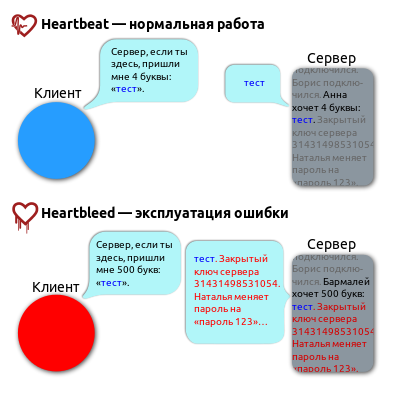
\includegraphics[width=\linewidth]{heartbleed}
\begin{center}
Рис. 1. Принцип использования уязвимости.
\end{center}

Уязвимость POODLE позволяет злоумышленнику отправлять свои данные на сервер по SSLv3 от имени жертвы, расшифровывать по 1 байту за 256 запросов. Происходит это из-за того, что в SSLv3 padding не учитывается в MAC. 

Теоретически, реализовать атаку можно на любой сервис, где есть возможность влиять на отправляемые данные со стороны атакуемого. Проще всего это реализовать, например, если злоумышленнику необходимо получить Cookie на HTTPS-странице, добавляя свой код на HTTP-страницы, который делает подконтрольные запросы на HTTPS-страницы, и подменяя шифрованные блоки.

\subsection{Практическое задание}

Выбрать со стартовой страницы SSL Server Test один домен из списка Recent Best и один домен из списка Recent Worst – изучить отчеты, интерпретировать результаты в разделе Summary

\paragraph{SSL Report: syndle.nl (141.138.202.120)}
~

Сервер защищен от down-grade атаки. Не использует слабозащищенных протоколов и алгоритмов. Небольшие "недостатки" касаются того, что сервер не поддерживает слишком старые версии аутентификации. Например для IE 6.

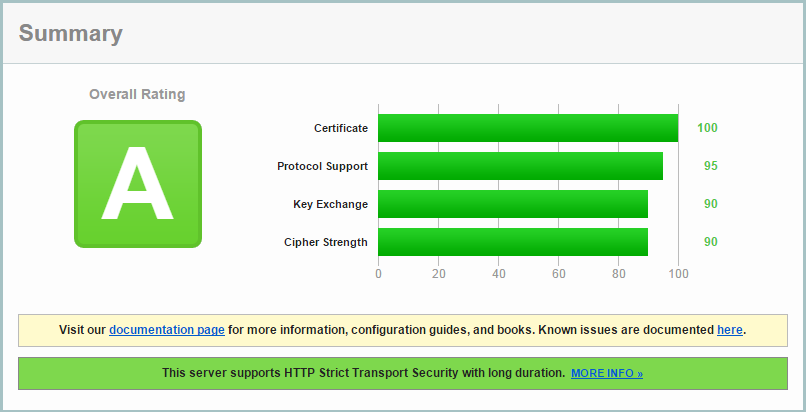
\includegraphics[width=\linewidth]{good}
\begin{center}
Рис. 2. Summary recent best.
\end{center}

\paragraph{SSL Report: sminc-owncloud.ddns.net (86.135.169.104)}
~

Данный сервер настроен похожим образом. Единственная его проблема то, что сертификат не подтвержден. Вероятно используется самподписанный сертификат. Однако это не является большой проблемой, если проект находится в процессе разработки.

\begin{center}
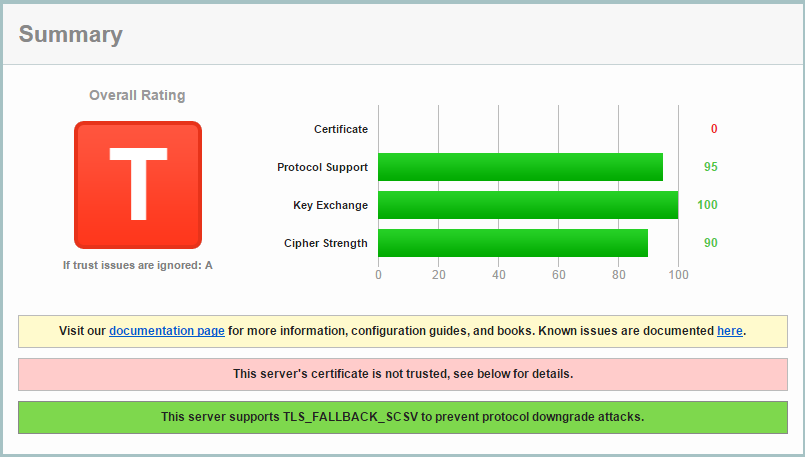
\includegraphics[scale=0.7]{bad}
\end{center}

\begin{center}
Рис. 2. Summary recent worst.
\end{center}

\paragraph{SSL Report: fwallet.tk (151.80.164.83)}
~

Для исследования был выбран сервер, используемый в текущем учебном проекте.
Данный сервер имеет ряд существенных недостатков:
\begin{enumerate}
\item Использование слабых параметров для алгоритма Диффи-Хелмана во время обмена ключами.
\item Сервер подвержен атаке POODLE, следует отключить SSL v3.
\item Сервер поддерживает алгоритм потокового шифрования RC4, который является недостаточно надежным.
\item Сервер не поддерживает Forward Secrecy, таким образом в случае утечки секретного ключа, данные пользователей могут быть расшифрованы.
\end{enumerate}

В то же время сервер не подвержен down-grade атакам.

\begin{center}
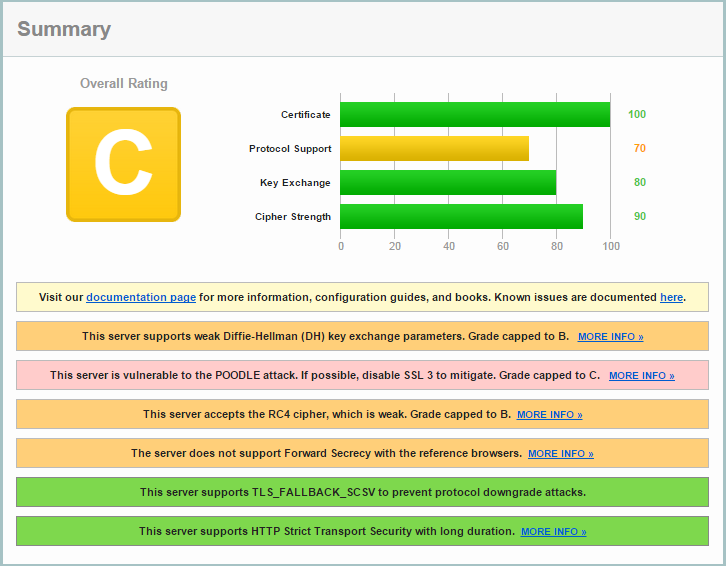
\includegraphics[scale=0.8]{custom}
\end{center}

\begin{center}
Рис. 3. Сервер, поддерживающий SSL/TLS.
\end{center}

\paragraph{Расшифровать все аббревиатуры шифров в разделе Configuration}
~

Каждая строка содержит информацию об используемых алгоритмах:
\begin{enumerate}
\item для обмена ключами
\item для шифрования сообщений
\item информацию о режиме шифрования
\item используемой хэширующей функции
\end{enumerate}

Для обмена ключами используются два алгоритма RSA и DHE(Diffie-Hellman Ephemeral).

Для симметричного шифрования данных используются алгоритмы RC4(потоковый алгоритм, слабозащищен), AES (все хорошо), camellia, SEED (на основе сетей фейстеля).

В качестве хэширующей функции используется SHA и SHA256 битный.

Также используются два режима шифрования CBC  (chaining block chiper) и GCM (Galois/Counter mode)
\small
\begin{verbatim}
TLS_RSA_WITH_RC4_128_SHA (0x5)   WEAK	128
TLS_RSA_WITH_AES_128_CBC_SHA (0x2f)	128
TLS_DHE_RSA_WITH_AES_128_CBC_SHA (0x33)   DH 1024 bits (p: 128, g: 1, Ys: 128)   FS   WEAK	128
TLS_RSA_WITH_CAMELLIA_128_CBC_SHA (0x41)	128
TLS_DHE_RSA_WITH_CAMELLIA_128_CBC_SHA (0x45)   DH 1024 bits (p: 128, g: 1, Ys: 128)   FS   WEAK	128
TLS_RSA_WITH_SEED_CBC_SHA (0x96)	128
TLS_DHE_RSA_WITH_SEED_CBC_SHA (0x9a)   DH 1024 bits (p: 128, g: 1, Ys: 128)   FS   WEAK	128
TLS_RSA_WITH_AES_128_CBC_SHA256 (0x3c)	128
TLS_DHE_RSA_WITH_AES_128_CBC_SHA256 (0x67)   DH 1024 bits (p: 128, g: 1, Ys: 128)   FS   WEAK	128
TLS_RSA_WITH_AES_128_GCM_SHA256 (0x9c)	128
TLS_DHE_RSA_WITH_AES_128_GCM_SHA256 (0x9e)   DH 1024 bits (p: 128, g: 1, Ys: 128)   FS   WEAK	128
TLS_RSA_WITH_3DES_EDE_CBC_SHA (0xa)	112
TLS_DHE_RSA_WITH_3DES_EDE_CBC_SHA (0x16)   DH 1024 bits (p: 128, g: 1, Ys: 128)   FS   WEAK	112
TLS_RSA_WITH_AES_256_CBC_SHA (0x35)	256
TLS_DHE_RSA_WITH_AES_256_CBC_SHA (0x39)   DH 1024 bits (p: 128, g: 1, Ys: 128)   FS   WEAK	256
TLS_RSA_WITH_CAMELLIA_256_CBC_SHA (0x84)	256
TLS_DHE_RSA_WITH_CAMELLIA_256_CBC_SHA (0x88)   DH 1024 bits (p: 128, g: 1, Ys: 128)   FS   WEAK	256
TLS_RSA_WITH_AES_256_CBC_SHA256 (0x3d)	256
TLS_DHE_RSA_WITH_AES_256_CBC_SHA256 (0x6b)   DH 1024 bits (p: 128, g: 1, Ys: 128)   FS   WEAK	256
TLS_RSA_WITH_AES_256_GCM_SHA384 (0x9d)	256
TLS_DHE_RSA_WITH_AES_256_GCM_SHA384 (0x9f)   DH 1024 bits (p: 128, g: 1, Ys: 128)   FS   WEAK	256
\end{verbatim}

\paragraph{Прокомментировать большинство позиций в разделе Protocol Details}
~

Первые три пункта касаются пересмотра сертификата и защищенности этого процесса.

Далее идет отчет об уязвимостях POODLE, BEAST и down-grade attack. 

Сообщение о том, что используется слабый алгоритм RC4.

Статус уязвимости heartbleed.

Предупреждение что Forward Secrecy не всегда работает.

Предупреждение о слабых параметрах алгоритма DH.

Совместимость с SSL v2 handhake.

\begin{verbatim}
Secure Renegotiation	Supported
Secure Client-Initiated Renegotiation	No
Insecure Client-Initiated Renegotiation	No
BEAST attack	Not mitigated server-side (more info)   SSL 3: 0x2f, TLS 1.0: 0x2f
POODLE (SSLv3)	Vulnerable   INSECURE (more info)
POODLE (TLS)	No (more info)
Downgrade attack prevention	Yes, TLS_FALLBACK_SCSV supported (more info)
TLS compression	No
RC4	Yes   WEAK (more info)
Heartbeat (extension)	Yes
Heartbleed (vulnerability)	No (more info)
OpenSSL CCS vuln. (CVE-2014-0224)	No (more info)
Forward Secrecy	With some browsers (more info)
Next Protocol Negotiation (NPN)	No
Session resumption (caching)	Yes
Session resumption (tickets)	Yes
OCSP stapling	No
Strict Transport Security (HSTS)	Yes   max-age=31536000; includeSubDomains
Public Key Pinning (HPKP)	No
Long handshake intolerance	No
TLS extension intolerance	No
TLS version intolerance	No
Incorrect SNI alerts	-
Uses common DH prime	Yes   Replace with custom DH parameters if possible (more info)
SSL 2 handshake compatibility	Yes
\end{verbatim}

\paragraph{Сделать итоговый вывод о реализации SSL на заданном домене}
~

Конфигруация сервера, обслуживающего данный домент сделана плохо, либо не сделана вообще. Сервер использует доверенный сертификат и защищен от некоторых атак (heart-bleed, down-grade, beast), однако все же содержит уязвимости (poodle, использование алгоритма RC4 и т.п.). Кроме того, сервер не поддерживает forward secrecy для всех браузеров, что является дополнительной угрозой. В качестве итога, можно сказать, что в случае необходимости специалист способен нанести значительный урон данному сервису. Таким образом, первичными задачами для исправления являются:
\begin{enumerate}
\item Настройка алгоритма DH
\item Отключение SSL v3
\item Отключение протокола RC4
\end{enumerate}

\section{Выводы}

В ходе данной работы были изучены "best practice" использования SSL/TLS. Были рассмотрены основные возможности сервиса Qualys SSL Labs – SSL Server Test. Данный сервис позволяет провести анализ качества защищенности домена. В качестве резюме можно получить статус самых известных уязвимостей для данной сервера, а также информацию о поддерживаемых протоколах и режимах работы. Кроме того, сервис тут же предлагает дополнительную информацию по вопросам решения указанных проблем. 

В качестве вывода, можно отметить важность анализа конфигурации SSL/TLS, особенно, при коммерческом использовании. Данный анализ можно удобно выполнить при помощи данного инструмента, однако если требуется особенно тщательная проверка, то она должна быть проведена дополнительно.
 
\end{document}